% \documentclass[superscriptaddress,showpacs,preprint,nofootinbib,11pt]{revtex4-1}
% %\documentclass[showpacs,pre,nofootinbib]{revtex4}
% %\usepackage{ulem}
% \usepackage{epsfig}
% \usepackage{bm}
% \usepackage{amsmath}
% \usepackage{subfigure}
% \usepackage{graphicx}
% \usepackage{epstopdf}
% \usepackage[pdftex]{color}
% \usepackage{hyperref}
% \hypersetup{
%     colorlinks=true,       % false: boxed links; true: colored links
%     linkcolor=cyan,          % color of internal links
%     citecolor=magenta,        % color of links to bibliography
%     filecolor=magenta,      % color of file links
%     urlcolor=cyan,           % color of external links
%     runcolor=cyan
% }
%
% \newcommand{\figurewidth}{0.8 \columnwidth}
% \newcommand{\beq}{\begin{eqnarray}}
% \newcommand{\eeq}{\end{eqnarray}}
% \newcommand{\bes} {\begin{subequations}}
% \newcommand{\ees} {\end{subequations}}
% \newcommand{\Tr}{{\text Tr}}
% \newcommand{\e}{{\text e}}
% \newcommand{\rmd}{{\text d}}
% \newcommand{\mc}{\mathcal}
% \renewcommand{\Re}{\operatorname{Re}}
% \renewcommand{\Im}{\operatorname{Im}}
% \newcommand{\bytroels}[1]{{\bf\textcolor{green}{#1}}}
% \newcommand{\byTA}[1]{{\textcolor{blue}{#1}}}
% \newcommand{\byJJ}[1]{{\textcolor{magenta}{#1}}}
% \newcommand{\byDL}[1]{{\textcolor{blue}{#1}}}
% \newcommand{\byIH}[1]{{\textcolor{cyan}{#1}}}
% \newcommand{\HI}{H_{\textrm{Ising}}}
% \newcommand{\pS}{p_{\textrm{S}}}
% \newcommand{\TTS}{\textrm{TTS}}
% \newcommand{\ignore}[1]{}
% \newcommand{\vs}{\textit{vs} }
% \newcommand{\red}[1]{\textcolor{red}{#1}}



% \begin{document}

% \chapter{Benchmarking or: How I learned to stop worrying and love Bayesian nonparametrics and optional stopping}

% \author{Joshua Job}
% \affiliation{Department of Physics and Astronomy, University of Southern California, Los Angeles, California 90089, USA}
% \affiliation{Center for Quantum Information Science \& Technology, University of Southern California, Los Angeles, California 90089, USA}
%
% \email{jjob@usc.edu}
%
%
%
% \date{\today}

% \begin{abstract}
% \label{ch:benchmarking}
Benchmarking is a difficult task, as partly discusse at the end of chapter \ref{ch:intro}, and if one does it naively one can easily fool oneself into believing false things with high confidence. In the hopes of aligning data analysis and data collection procedures across our community, this chapter presents a basic overview of the effects of gauges, the modeling of benchmarking time to solution (TTS) for algorithms for Ising-type problems, Bayesian nonparametric modeling, and applies the insights learned to the benchmarking problem. The final procedure for data analysis is quite similar to previous methods, while the data collection procedure is quite different.

 In general, the conclusion for quantum annealers is that one should collect $\approx$100 anneals for each programming cycles/gauge, unless there is a specific reason to change it, and continue running until the coefficient of variation of one's posterior distribution for probability of success or TTS falls below a threshold of 0.2 (or 0.1). Estimates of the posterior should be performed by drawing samples from the distribution defined by first sampling a value from each gauge's posterior distribution for $p_s$, Beta$(x,100-x)$ for $x$ successes in that gauge, and then performing a weighted average with weights drawn from the Dir(1,1,1,...,1) distribution (a Bayesian bootstrap).
% \end{abstract}


% \maketitle

The development of the D-Wave line of quantum annealers has sparked a flurry of activity in the optimization and quantum computation community, and spurred a small cottage industry around benchmarking their performance. This chapter is not concerned with the results of any such analysis, but with the method of analysis itself. The goal is to lay out guidelines which will hopefully aid all future researchers in this field benchmark future generations of D-Wave devices, as well as competing optimization algorithms, in a consistent and standard way.

This chapter is organized into three parts. The first addresses the problem of data analysis alone, introducing the benchmarking problem formally again and discussing the ideal solution as well as realistic solutions forced upon us by practical necessities. It includes a brief introduction to the field of Bayesian nonparametrics and its bread and butter, the Dirichlet distribution and the associated Dirichlet process, and grounds the analysis procedure in this field, while exploiting a technique which is simpler computationally called the Bayesian bootstrap. It concludes with a comparison between the Bayesian and classical bootstraps, arguing that the classical bootstrap is conceptually flawed and computes a distribution we, as scientists, don't care about (the sampling distribution of a statistic) while the Bayesian bootstrap gives us the distribution we typically think the classical bootstrap gives us --- namely a posterior distribution on the parameter or function of interest.

The second part addresses the question of data collection procedures, and outlines an approach based on optional stopping, where one uses the data itself to determine when one has enough data, on the fly, instead of specifying sample sizes in advance. While this has the downside of resulting in an estimator with a small bias, this bias is controllable (it decreases linearly with the number of gauges sampled), small (a few percent at most), and acts effectively as an overall constant factor on the TTS rather than as an element with scaling. It thus has no bearing on scaling results, which involve fitting to an exponential. Moreover, the resulting posterior credible intervals have very good frequentist coverage properties. The chief benefit is a potentially enormous time savings when one seeks to learn the TTS for most instances in a collection.

The third section presents the conclusions of a simulation study using various artificial distributions meant to highlight various possible cases and to validate the collection procedure and recommendations given in the rest of the paper.

A few notes on style before we begin: First, this paper is written in a tone more similar to a presentation than a traditional paper. Second, I use ``I'' throughout to refer to the author, and ``we'' to denote ``the reader and I''. It is also rather opinionated. As this chapter has not appeared in any form in a publication, and as it was wholly original and written solely by the author of this dissertation, it will likely be the most idiosyncratic chapter.

\section{Please lie down on the couch: Data analysis}
\label{sec:bp}
Suppose that you have a problem, $H$ whose properties depend on some set of parameters which you control, call them $\lambda$, as well as a set of nuisance parameters $\theta$ you do not control and/or do not care about. A solver takes in some problem $H(\lambda,\theta)$ and outputs a trial solution $\vec{s}$ under some set of solver parameters $\chi$. We have some function $\Phi$ which maps a solution $\vec{s}$ into a binary output $s=0,1$ for ``failure'' and ``success'' respectively. Note that this language may be misleading --- any binary classifier on the samples $\vec{s}$ qualifies. Applying the map to all solutions sampled from the solver, and we can represent a solver as a simple generator of a sequence of 0s and 1s.

The problem of interest is to learn the probability under some defined distribution over the parameters $\theta$ that a given solution will be classified as a ``success'' or 1. In other words, we seek to estimate $p_s(\lambda,\chi) = \langle Pr(s=1|H(\lambda,\theta),\chi) \rangle_\theta$, and thus also the time to solution (related to $p_s$ through a nonlinear transformation $log(0.01)/log(1-p_s)$, as defined in previous chapters).

Here, $\lambda$ could be the list of all couplers specifying the Hamiltonian, but it could also include meta-parameters such as the range of random Ising problems, the loop density in the frustrated loop planted solutions, chain strength in an embedded problem, etc. Any property of an instance which, contextually, we wish to account for and track explicitly. The $\theta$ constitute variables to be averaged over, like the physical couplers of the programmed Hamiltonian (which are inaccessible and taken to be stochastic).

Certain properties may lie on either side of this boundary depending on context. If one is studying the correlation between particular embeddings of full connected problems into Chimera, then embeddings would be in $\lambda$. If one instead simply views different embeddings as different but effectively equal representations of the same underlying problem, then the embedding would be in $\theta$. Variables like annealing time, number of sweeps, initial and final temperature, number of replicas in parallel tempering, number of Trotter slices in PIMC, etc. constitute $\chi$.

The task of benchmarking perfomance on a particular instance is, to repeat in this language, to estimate $p_s(\lambda,\chi)$, or, for fixed $\chi$, simply $p_s(\lambda)$.

\subsection{Paradiso: the ideal solution}
If one resamples $\theta$ for each trial according to its intrinsic distribution, then the expected probability of success at any trial is exactly $p_s$ (this is, indeed, what it means to ``marginalize'' over a variable, i.e. to average over it). By resampling $\theta$, we effectively render the success or failure of each new solution a simple Bernoulli trial. We then seek to estimate the probability of success of this Bernoulli trial. To do so, the default procedure is to choose a conjugate prior to the Bernoulli distribution, namely a Beta distribution, and update via Bayes rule on the evidence from repeated trials. Conjugate priors have the helpful property that the posterior distribution will be of the same family as the prior after updating on new evidence \cite{jaynes2003probability}. For the Beta distribution with a prior $Beta(c_1,c_2)$ and a sequence of N trials with x successes, the posterior is simply $Beta(x+c_1,N-x+c_2)$. $c_1$ can thus be considered the prior's number of pseudosuccesses and $c_2$ the prior's number of pseudofailures.

This can be immediately seen, as the probability density $p$ of $Beta(\alpha,\beta)$ is $p\propto p^{\alpha-1} (1-p)^{\beta-1}$, and the likelihood of observing $x$ successes from a Binomial random variable in $N$ trials is simply $\propto p^{x}(1-p)^{N-x}$.

To review for those unfamiliar with Bayesian terminology, a \textbf{prior} is one's initial information or state of belief about a value, and a \textbf{posterior} is one's information after adjusting one's views according to the rules of probability after acquiring new information.

The choice of prior has negligible impact to the posterior distribution when $c_1 \ll x$ and $c_2 \ll N-x$. Generally, $c_1=c_2=c$, and there are three common choices each with arguments in its favor -- $c = 0$, $\frac12$, or $1$. $c=1$ is the uniform distribution on $[0,1]$. $c=\frac12$ is the arcsine distribution, and is the Jeffrey's prior for the Bernoulli/Binomial distribution, namely the prior which is the square root of the determinant of the Fisher information matrix (and is thus invariant under reparameterization of the distribution). Finally, $c=0$ is the Haldane prior, which is a half-delta function at 0 and another at 1. The Haldane distribution is the only one for whom the mean of the posterior is equal to $x/N$, in general it is equal to $\frac{x+c_1}{N+c_1+c_2}$ for a $Beta(c_1,c_2)$ prior. The standard deviation is $\big(\frac{(x+c_1)(N-x+c_2)}{(N+c_1+c_2)^2(N+c_1+c_2)}\big)^\frac12$. The coefficient of variation, $\sigma/\mu=\sqrt{\frac{N-x+c_2}{(x+c_1)(N+c_1+c_2)}}$. If $c_1$ and $c_2$ are small relative to $N-x$ and $N$, this is approximately $\frac1x-\frac1N$, and for large $N$ is just $\frac1x$.

We immediately see an important lesson: the coefficient of variation of $p_s$ is controlled by the number of successes that we see. Thus, if we wish to estimate to within a fixed variation, we require the number of successes to be approximately constant.

\subsection{The realistic solution}
While a method of operation like the above is available to us for some algorithms (those on classical hardware for instance), to resample $\theta$ at each trial on D-Wave hardware is untenable due to the long programming time. If run in such a mode, the D-Wave chip will be annealing only $\approx 1\%$ of the time. In a given time $T$, one can perform $G=T/(\tau_{prog}+\tau_{anneal} R)$ gauges where $\tau_{prog}\approx 15ms$ is the programming time per gauge, and $\tau_{anneal}\approx 150ms$ is the total time per anneal (including readout). For $R=1$ you can perform approximately $66$ gauges per second with $66$ samples. For $R=100$ you can perform approximately $33$ gauges per second with $3300$ samples, and for $R=200$ you can perform approximately $22$ gauges with $4400$ samples. One sees there is a shift, from a moderate decrease in the number of gauges causing enormous increases in the number of samples (and thus better probability estimates) to moderate tradeoffs in the number of gauges corresponding to moderate increases in the number of samples. For $R>1000$ this tradeoff is quite catastrophically large, moving from $R=1000$ to $R=50000$ increases the number of samples per second by less than $10\%$ while decreasing the number of gauges per unit time by roughly a factor of $50$. Since we have no interest in the individual probability per gauge except what it tells us about the mean over $\theta$, we should expect that restricting ourselves to $R\approx 100$ will yield the most efficient inferences. Later simulation studies will show that quite generally $R=100$, i.e. that $R$ such that the quantum annealer spends approximately half of it's time programming and half annealing, is indeed the optimal number of runs per gauge for our probability estimates to converge with the minimum wall-clock time, i.e. the minimum effort. Thus, out of practical necessity we must perform multiple trials from each value of $\theta$ and then take an average to estimate $p_s$.

For each set of trials (equivalent to a programming cycle on the D-Wave processor; I will call them ``progcycles'' or ``gauges'' interchangeably) we can use a Beta distribution to encode our knowledge about the probability of success for that progcycle, and then compute our belief about the average value over all progcycles. Now, the choice of prior is no longer practically irrelevant (unlike the ideal case). Since we know we cannot run an unlimited number of anneals with a single progcycle we will inevitably reach a point where the overwhelming majority of our progcycles have zero successes. If our prior on $p_{success}$ for a gauge has any bias in the average value, then we'll have a bias of the same magnitude in our estimate for the average, $p_s$. Thus, for very difficult problems, with low success probabilities, our prior will swamp our data and we will learn nothing no matter how many anneals we perform. Thus, we are forced to choose the Haldane prior, $Beta(0,0)$, for the prior on the probability of success of each gauge, as it is the only Beta distribution prior whose mean is equal to the empirical success rate and thus is not biased by prior information.

\subsection{I was blind but now I see: Bayesian nonparametrics}

We can construct a Bayesian model for our problem: $Y_i \sim Bin(R,p_i)$ are the number of successes for each progcycle $i$ given some probability of success $p_i \sim F$ for some unknown distribution $F$. To complete a full Bayesian model specification, we must specify a prior on $F$. This may at first seem quite difficult, even impossible, as $F$ can in principle be any probability distribution defined on the interval $[0,1]$. Moreover, if the prior isn't conjugate it may be infeasible to compute posterior densities. There is, however, a density which is conjugate to iid sampling, and it is called the Dirichlet process.

\subsubsection{The Dirichlet Distribution}

Before discussing the Dirichlet process (DP) in more detail, allow me first to quickly introduce a related distribution: the Dirichlet distribution. Denoted by Dir$(\vec{\alpha})$ for an arbitrary vector of positive real parameters $\vec{\alpha}$, the Dirichlet distribution is conjugate to the categorical and multinomial distributions.

Suppose you wish to estimate the probability of rolling each side of a six-sided die. Just as for the Beta distribution there are a set of common choices of prior Dirichlet distribution priors. The one whose mean corresponds to the maximum likelihood estimate (MLE) is the one with all 0s in $\vec{\alpha}$ \cite{rubin1981bayesian}. The posterior with this prior, assuming one saw $x_i$ instances of the number $i$ after a total of $\sum_i x_i = N$ rolls of the die will be Dir$(x_1,x_2,x_3,x_4,x_5,x_6)$. The marginal density for $p(i|\vec{x}) = $Beta$(x_i,N-x_i)$, peaked at the empirical probability of success. The resulting posterior density will be a smooth version of the posterior derived from the classical bootstrap (which is discussed later, but is simply resampling values from your empirical distribution \cite{efron1992bootstrap}).

An important property of the Dirichlet distribution is that one can repartition the space of outcomes and the result will still be Dirichlet. For instance, the distribution of ``(1 OR 2), 3, 4, 5, 6'' would be given by Dir$(x_1+x_2,x_3,x_4,x_5,x_6)$ (while the corresponding conditional distribution just on 1 and 2 would be Dir$(x_1,x_2)$). This ability to regroup elements in the space of outcomes at will and easily compute marginal distributions is one of the reasons why the Dirichlet distribution and it's extension, the Dirichlet process, are so useful in Bayesian statistics.

The Dirichlet process was originally proposed in \cite{Ferguson:1973}. Since, there have been a number of characterizations of it, but for our purposes here we need only deal with the first. A Dirichlet process DP$(\alpha F_0)$ is a probability distribution on the support of the ``base distribution'' $F_0$ that is almost surely discrete. It has the property that for any partition of the support of $F_0$, call it $(X_1,X_2,...,X_N)$, one finds that realizations $F$ of $DP(\alpha F_0)$ obey the following property: \[(F(X_1),F(X_2),...,F(X_N)) \sim Dir(\alpha F_0(X_1),...,\alpha F_0(X_N))\], where $A(X)$ denotes the total support of whatever distribution $A$ on the interval $X$. This rule applies for every partition $\{X\}$ simultaneously. While at first it is not obvious such a process is possible, it is and it is actually fairly trivial to sample realizations to arbitrary accuracy from a Dirichlet Process.

The Dirichlet process is conjugate to iid sampling. If one samples a set of $N$ values from $F$ $\{\theta_i\}_{i=1}^N$, one's posterior distribution for $F$ is DP$(\alpha*F_0+\sum_i \delta_{\theta_i})$, where $\delta_\theta$ denotes an atom with weight 1 on the point $\theta$. Thanks to the above partitioning property, one can rewrite this (at least to arbitrary accuracy) as \[\mathrm{DP}\big(\alpha*F_0+\sum_i \delta_{\theta_i}\big) = p*\mathrm{DP}(\alpha F_0) + (1-p)\mathrm{DP}\big(\sum_i \delta_{\theta_i}\big)\] \[p \sim \mathrm{Beta}(\alpha,N)\] by separating the points $\{\theta_i\}$ and arbitrarily small regions around each point into one partition and the rest of the interval (which is effectively the entire interval, minus $N$ holes) into another. The distribution DP$(\sum_i \delta_{\theta_i})$ is quite interesting, in that it effectively only has support on a finite set of points. Indeed, it is identical to a Dir$(\vec{1}^N)$ ($N$ 1's) distribution on the collection of points $\theta_i$. We will return to this distribution shortly. (Note, to my knowledge this is actually an original representation of the posterior of a DP.)

What role do $\alpha$ and $F_0$ have? $\alpha$ acts as a strength parameter, essentially representing how confident we are that the true distribution is in the ``vicinity'' of $F_0$. If $\alpha$ is very large, it will take quite a lot of data for the data to overwhelm the prior (as seen from the weights between the components of the posterior, namely $Beta(\alpha,N)$). If $\alpha$ is very small, the prior has negligible influence on the posterior estimates even at small sizes. In the limit $\alpha\rightarrow 0$, the distribution becomes purely the above Dir$(\vec{1}^N)$ on the points $\{\theta_i\}$. This distribution has been given another name, the Bayesian bootstrap, introduced in Ref \cite{rubin1981bayesian}, and will henceforth be denoted as $BB(\vec\theta)$ The Bayesian bootstrap has no free parameters, and is wholly determined by the data vector $\vec\theta$. One can see that the Bayesian bootstrap also dominates the Dirichlet Process in the limit of $N\rightarrow\infty$.

With all these preliminaries in mind, we can complete our Bayesian model specification as
\begin{align*}
	Y_i &\sim \mathrm{Bin}(R,p_i) \\
	p_i &\sim F \\
	F &\sim \mathrm{DP}(\alpha F_0)
\end{align*}
for some values of $\alpha$ and $F_0$ denoting our prior beliefs (which may, in principle, vary from person to person). This problem was actually investigated in \cite{BerryChristensen1979}, where they computed an approximation to the true posterior distribution. \cite{Kuo1986a} demonstrated an importance sampling technique to attempt to approximate the posterior for conjugate priors $F_0$. In the last two decades, additional MCMC techniques have been developed for inference in the general case for Dirichlet processes \cite{gelfand2002}.

These have several disadvantages, however. First and foremost, these MCMC approaches are generally quite slow to converge, and indeed can take minutes, hours, and even days when one has tens of thousands of data points (as would be the case for benchmarking fairly hard problems, with success probabilities in the $10^{-5}$ range). This is simply impracticle for our datasets. A number of approximation techniques have been proposed, such as \cite{Wang2011}.

Approximations don't overcome the other challenge, however, which is eliciting sensible prior values for $\alpha$ and $F_0$. Often researchers place hyperpriors on these, and learn their values, too, from the data, but this only makes the convergence problem of the MCMC algorithms worse. Moreover, our community is not composed solely of Bayesians, and soliciting good priors is a notoriously difficult problem in any case. Rather than attempt to do so, it is my suggestion that we instead adopt the Bayesian bootstrap directly as our inference mechanism.

\subsection{Why the Bayesian bootstrap?}

This is justified in several ways. First and foremost, the Bayesian bootstrap is the only way the data enters into the posterior of the Dirichlet process for a given sample from $F$ $\vec\theta$. Since our prior will obviously be weak (as we don't have any good idea of what $F$ should look like \emph{a priori}), and we will want to take a large amount of data in any case, the posterior will  likely be very near the Bayesian bootstrap anyway. $\alpha\rightarrow 0$ serves as a fairly natural noninformative prior for Dirichlet processes, acting in a manner similar to the Haldane and Dir$(\vec 0)$ priors for Binomial and Multinomial distributions.

Finally, this prior is extremely tractable and flexible. Since we know that each element of $\vec \theta$ must be distinct (as they are simply the true probabilities of success for each gauge we ran and the underlying distribution is almost surely continuous and nonatomic), we can treat each $\theta_i$ independently, deriving a posterior distribution for each and then performing a Monte Carlo average. The posterior for $\theta_i$ is Beta($x_i,R-x_i$) given a Haldane prior, which also corresponds to taking the likelihood function $L(x_i|\theta_i)$ and interpreting it as a distribution on $\theta_i$. We would then place a Dir$(\vec{1})$ distribution on the weight of each sample in our posterior estimation. That is:

\begin{align*}
\theta_i &\sim \mathrm{Beta}(x_i,R_i) \\
w_i &\sim \mathrm{Dir}(1,1,1,...,1) \\
p_s &= \sum_i w_i \theta_i
\end{align*}


MC simulations of this type can be performed in seconds even with tens of thousands of data points, making them suitable for use in online learning of our parameters and their credible  intervals. Indeed, due to the decomposition property of the Dirichlet distribution, one can even update an existing ensemble of points sampled from one's posterior to update to a new sample from one's posterior on the acquisition of new information, leading to effective sample times of well under a second for thousands of realizations.

Let us imagine that for some problem, $x=R$ or $x=0$ for all of $N$ gauges run. If $x=R$, one's posterior for $\theta_i$ is a delta function at $1$, while for $x=0$ it is a delta at $0$. As a result, one can regroup elements in the Dirichlet distribution into ``deltas at 0'' and ``deltas at 1'', yielding Dir$(N-X,X)$, where $X$ being the number of gauges with all 1s. The sampled values from $p_s$ will then be $(1-p)$ for $p\sim \mathrm{Beta}(N-X,X)$, i.e. Beta$(X,N-X)$. Notice that if one sets $R=1$, one is actually performing the ideal experiment and the analysis procedure yields a posterior that is exactly the posterior for the ideal case (with a Haldane prior). This is an extremely attractive feature, and another source of justification for using the Bayesian bootstrap.

How does the Bayesian bootstrap compare to the classical bootstrap?

\subsection{To Bayes, or not to Bayes, that is the question: Bayesian v. classical bootstrap}
While the Bayesian bootstrap has a natural connection to Bayesian non-parametrics, it isn't obvious what the payoff is over the classical bootstrap unless one is a committed Bayesian and frequentism makes one queasy. Why bother when we already have the classical bootstrap if they're so similar? To explain the differences, let's review the classical bootstrap and compare the assumptions each bootstrap makes.

In a classical bootstrap \cite{efron1992bootstrap}, one makes the following assumptions:
\begin{enumerate}
	\item All values that may be sampled from the distribution have been. (One has seen every type in the population.)
	\item All frequencies of the types in the population are exactly those in the empirical sample.
\end{enumerate}

One then estimates the distribution for a parameter of interest under these assumptions. One does so by creating new pseudodata vectors by sampling with replacement $N$ values from the original vector (of length $N$).

A key point is that the classical bootstrap mimics the \emph{sampling} distribution of a parameter, not the distribution of the parameter in the population. In the case of benchmarking this distinction proves fatal for the classical bootstrap. Take, for instance, the case where one has $10$ gauges, $9$ of whom have $0$ successes and 1 of whom has all successes, after $R$ trials in each gauge. We know the Bayesian bootstrap will yield Beta($1,9)$ as discussed above. For the classical bootstrap, we would be sampling from $\frac1n \mathrm{Bin}(10,0.1)$. A plot of this is provided in \ref{fig:cbsucks}.

\begin{figure}[hbt]
  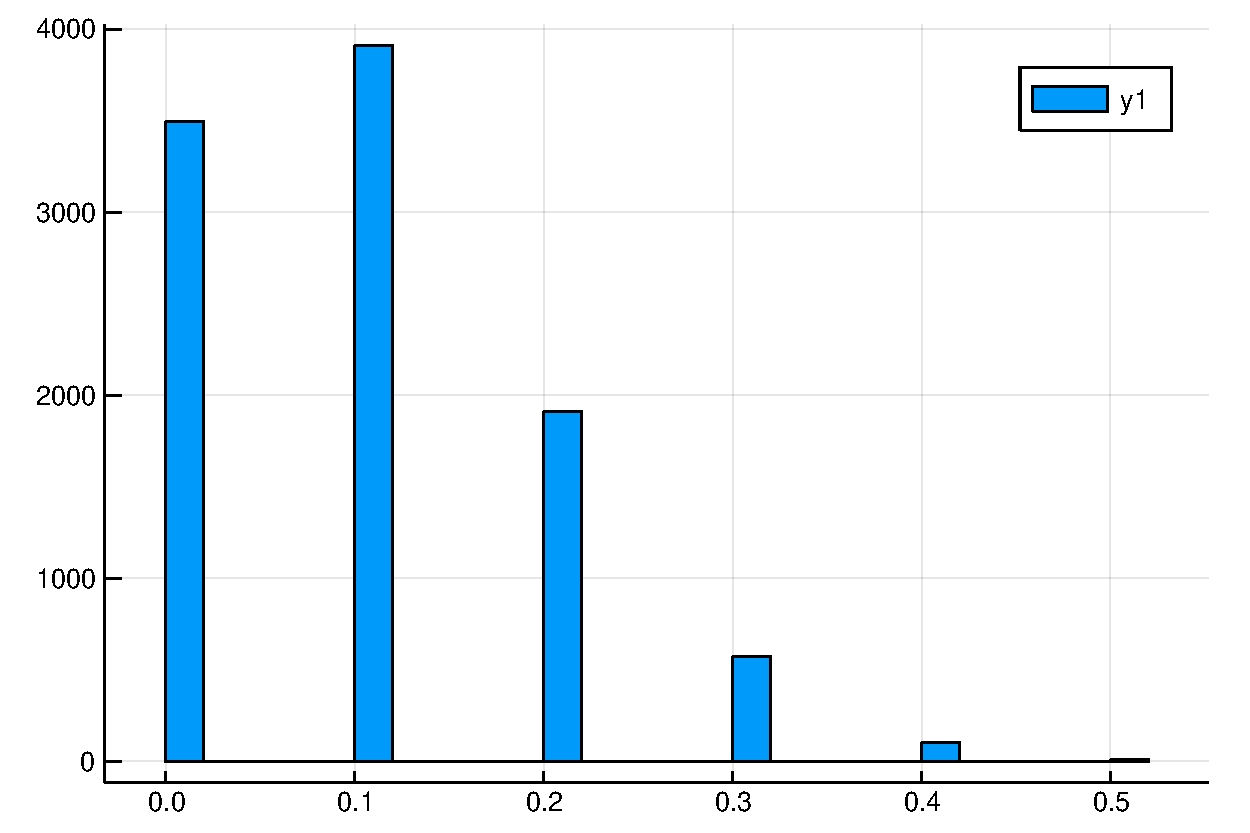
\includegraphics[width=\columnwidth]{chapters/Benchmarking/cbsucks}
  \caption{Results from 10000 frequentist bootstrap samples from a sample of 10 gauges, nine with zero successes and one with all successes. If one tried to interpret this as a distribution of one's uncertatiny about the mean success probability, averaged over all gauges, then one has significant weight on the mean success rate is 0, even though one actually observed successes, a clear contradiction.}
  \label{fig:cbsucks}
\end{figure}

As you can see, you have non-negligible support on $p_s=0$. But of course, this isn't $p_s$, the gauge-marginalized mean success probability, this is our bootstrapped estimate of the sampling distribution for our statistic. The practitioner of the classical bootstrap is left with few options when attempting to move to sampling from the distribution for time to solution, which goes like $1/p_s$ and thus has weight on TTS$=\infty$. Any time there is a gauge with all zeros, the classical bootstrap will place support on infinite time to solution, whether we happen to have sampled those elements from the distribution or not. Thus, while we may be able to ``get away with it'' in the sense that using the classical bootstrap won't always fail in practice due to the presence of a single $0$, the fact remains that we know analytically the true mean of the bootstrap estimate for $TTS$ is $\infty$.

This gets to a deeper issue: if the classical bootstrap is supposed to somehow represent my knowledge or information about $p_s$, then it clearly fails. We have seen successes, yet the frequentist bootstrap places nonzero weight on the belief that the average probability of success is $0$, and thus observing a success is impossible. But I've seen one. More than one in fact! It strikes one as incredibly odd that one would use a procedure which seems to predict that there is a chance one couldn't possibly have observed a value one did, in fact, observe.

Fundamentally, we aren't interested in the sampling distribution of our parameter of interest; we're interested in learning about the parameter itself, i.e. a posterior distribution, which is quite different conceptually and, as one will see, in practice. Often, statisticians can get away with ignoring the difference, but one does so at one's own peril (such as by attempting to produce a scaling plot of TTS and having an error bar that goes to $\infty$).

One may still counter ``So long as the weight on 0 is small enough, it won't matter for practical purposes.'' To couch the differences in a more pragmatic context, consider also the case where we have $100$ gauges (normally considered plenty for problems with appreciable probability of success in our field, say $p_s>0.01$), each with $2000$ anneals, and a distribution of probability of success chosen from a mixture of Normal$(0.05,0.003)$ with weight $0.95$ and Normal$(0.4,0.01)$ with weight $0.05$, and observe what the classical bootstrap has to say about $p_s$ in this case as well \ref{fig:pointy}

\begin{figure}[hbt]
  \includegraphics[width=\columnwidth]{chapters/Benchmarking/pointy}
  \caption{Results from 1000 frequentist bootstrap samples from a set of 100 gauges whose success probability was sampled from a mixture distribution of Normal$(0.05,0.003)$ with weight $0.95$ and Normal$(0.4,0.01)$ with weight $0.05$. The multiple peaks arise from the discrete binomial distribution over samples from the high probability component.}
  \label{fig:pointy}
\end{figure}

As you can see, the sampling distribution has a number of peaks which one would not expect from a posterior distribution for a mean. These arise due to the discrete nature of the classical bootstrap --- in each sample, the bootstrap has sampled a certain discrete number of the large-mean distributions. The variation in the number of samples from Normal$(0.4,0.01)$ overwhelms the variation over the other samples, effectively creating a Binomial distribution on the number of said gauges with Gaussian noise from the other gauges centered on each discrete value.

While this example can be ``fixed'' by simply collecting more data (in this example, $200$ gauges would be approximately sufficient), the fundamental problem will remain --- frequentist statistics estimate uncertainty due to sampling, not our uncertainty about parameters themselves.

Rubin \cite{rubin1981bayesian} proposed the Bayesian bootstrap. It can be understood (entirely separate from the above derivation from the Dirichlet process) as based on two assumptions:

\begin{enumerate}
	\item All values that may be sampled from the distribution have been. (One has seen every type in the population.)
	\item The true population distribution is unknown. We merely have sampled G times and seen all G types (as per 1).
\end{enumerate}

To encode (2) mathematically, we recall that the conjugate prior to the categorical and multinomial distributions is the Dirichlet distribution (whose equivalent of the Haldane prior is Dirichlet$(0,0,0,0,0,...)$). Thus, if we take the standard prior for the G-dimensional Dirichlet distribution and update based on having seen each type once, we get the Dir$(1,1,1,1,...,1)$ distribution (for convenience, we will refer to this distribution as Dir$(\vec{1})$ where the dimension is implicit), aka the Bayesian bootstrap as defined above from DPs. Rather than sampling a vector of finite length at each sample as in the classical bootstrap, one samples from the Dirichlet distribution to find the weights for each element in the population to get a trial population on which to compute whatever statistic one desires.

The major practical benefit of the Bayesian bootstrap is that it yields continuous results for the mean for any continuous probability distribution, and has zero weight on all probability densities which have zero weight on an observation --- that is, if you observed a success, the Bayesian bootstrap will never sample $p_s=0$. It also has a more reasonable assumption than the classical bootstrap --- rather than asserting certainty about the distribution in the population, it assumes that we are ignorant of this distribution and uses only the knowledge we have. Finally, rather than representing some sampling distribution for a statistic, we are computing a genuine posterior distribution for our information about the statistic.

Let's examine the cases where the classical bootstrap broke down again, to see the advantages of the Bayesian bootstrap. In the case of 10 gauges with 9 having no successes and one having only successes, as discussed above, the posterior will be Beta(1,9). Beta(1,9) has no support on 0, i.e. there is no weight on $TTS=\infty$. The Bayesian bootstrap never claims it may be impossible to observe observed values.

In the second case, we have the result in figure \ref{fig:pointy_BB}.

\begin{figure}[hbt]
  \includegraphics[width=\columnwidth]{chapters/Benchmarking/pointy_BB}
  \caption{Results from 10000 Bayesian bootstrap samples from a set of 100 gauges whose success probability was sampled from a mixture distribution of Normal$(0.05,0.003)$ with weight $0.95$ and Normal$(0.4,0.01)$ with weight $0.05$. It is now a smooth density, unlike in the frequentist case.}
  \label{fig:pointy_BB}
\end{figure}

As one can see, this is smooth and continuous, due to the continuous nature of the Bayesian bootstrap, which is also a far more reasonable posterior distribution for a mean.

The Bayesian bootstrap can be nested, just like the classical bootstrap. For instance, one may desire to compute the posterior for the median over a class of instances, such as range-1 random Ising problems for $C_8$ chimera graphs. To do so, for each instance sample a value from the Bayesian bootstrap distribution for $p_s$. Then, compute the median over a population with those values of $p_s$ with population weights sampled from the Dir$(\vec{1})$ (this may be very different than the median over the vector of sampled $p_s$ alone) to extract a single sample of the median, and repeat many times to construct a Monte Carlo estimate of the posterior for the median. In general posteriors estimated in this way will be significantly smoother than estimates generated from the classical bootstrap, though may still be multimodal by the essentially discrete nature of order statistics on finite populations.

So long as the practitioner doesn't want weight on the problem being impossible after having solved it or expects posterior estimates of means to be smooth and unimodal (i.e. everyone) then the practitioner should use the Bayesian bootstrap rather than the classical bootstrap.

Now that we know how to estimate $p_s$, it is time to draw this paper to a close. Given an arbitrary distribution we have a technique to estimate $p_s$ and the benchmarking problem, at least as stated above, is solved. But a way to analyze data you already have isn't really a full solution to the real benchmarking problem. We know what to do if someone hands us a collection of data. But our goal is to perform an investigation ourselves. How should one go about collecting the data in the first place?

\section{Goldilocks and the three samples sizes: why there is no universal ``right'' sample size}
Traditionally in science, particularly in frequentist circles, scientists are admonished to design an experimental protocol in advance, including selecting sample sizes. This is due to concerns over the possibility of induced bias in estimates under conditions of ``optional stopping'', i.e. determining sample sizes by peeking at the data as you go along. Indeed, the debate about optional stopping has raged for over fifty years.

Why are sample sizes usually determined in advance? A simple stopping rule can point out how optional stopping could lead to incorrect inferences: continue sampling until such time as you can reject your null hypothesis with a p-value of 0.05. Obviously, this rule will cause you to always reject the null hypothesis, even if it's true, as for any distribution there is a remote possibility of sampling a chain which would satisfy it. This proposal was given by Armitage at the Savage Forum in 1959 \cite{mayo2001}, and has been the topic of quite a bit of debate since.

Nevertheless, despite the potential dangers of optional stopping, it has one dramatic advantage for the cause of benchmarking: it allows us to run relatively few samples for easy problems, and only run many samples for problems which are very hard. This could, in principle, enormously reduce the time to gather sufficient statistics.

To gauge how significant the time savings may be, recall that we expect the number of observed successes to control the accuracy of our inference, namely we suspect that number of gauges $G \propto 1/p_s$. We can examine the distribution over $p_s$ for problems of interest and it's scaling as a function of system size to approximately determine the time savings. One can see in Figure \ref{fig:optstop}, which shows approximately how many gauges would be necessary to complete gathering all data for various sizes of range-1 Ising problems tested in chapter \ref{ch:speedup}, assuming we wish to solve at least 95$\%$ of them (which seems a reasonable number). As one can see, optional stopping would reduce the time to gather all data by roughly an order of magnitude for the largest system size. These benefits should be expected to compound as we go to larger systems, with a broader distribution for $p_s$ across instances. Given that problems are also going to get exponentially harder, requiring longer data collection times, this could serve as an enormous practical reduction in difficulty.

\begin{figure}[hbt]
  \includegraphics[scale=0.66]{chapters/Benchmarking/optionalstoppingsavings}
  \caption{A comparison of the approximate number of gauges required to gather sufficient data to know TTS for the easiest $95\%$ of instances for various sizes of range-1 Ising problems. Optional stopping consumes more than an order of magnitude less time for the largest size, and we should expect this advantage to continue to grow as we go to larger systems with broader distributions for $p_s$.}
  \label{fig:optstop}
\end{figure}

Given that we desire to use some optimal stopping rule, how might we go about selecting one?

First, it seems natural to perform inference in TTS space, as that is the space that (a) correlates with how long it takes to gather the data and (b) is the space in which costs are directly proportional, rather than connected by a nonlinear function as in $p_s$ space. Thus, we convert our posterior densities on $p_s$ to TTS before applying whatever stopping rule we wish. Since we want to have a large amount of information about the value of TTS, we will place a threshold on the posterior coefficient of variation (equal to $\sigma/\mu$ for standard deviation $\sigma$ and mean $\mu$), such that we will stop gathering data once our estimated posterior $\sigma/\mu < c$ for small $c$.

This stopping rule corresponds directly to placing a threshold on the number of successes in the ideal $R=1$ case. Such a stopping rule was analyzed in \cite{Mendo2006} and found to be virtually unbiased (with a bias upper bounded by $-1/N$ where $N$ is the number of successes; this corresponds to a threshold $c=1/\sqrt{N}$ in the ideal case) with guarantees on the confidence level (essentially, resulting from $c$). While I was unable to make significant progress in analyzing the non-ideal $R>1$ case analytically, simulation studies detailed below will demonstrate that this proposed stopping rule is also virtually unbiased and has extremely good frequentist coverage properties (indeed, the credible intervals are often overly conservative, which could be a good or a bad thing depending on your point of view --- it's either somewhat wasteful or good protection against being overconfident).

Before we see those results, what properties do we expect of this stopping rule? By the law of large numbers we expect the posterior standard deviation to decrease like $\approx 1/\sqrt{G}$, and thus for the number of gauges to be roughly inversely proportional to the square of the threshold. Thus, the bias term decreases quadratically, with inverse $c^2$, as do the number of gauges. $G \propto \frac1\mu$, as would be expected. In general, we expect $G$ to also grow as the inverse square of the coefficient of variation of the underlying distribution.

\section{The proof is in the pudding: a simulation study}
To study the entire above procedure's performance, we perform a simulation study. The data collection algorithm is as follows:
\begin{enumerate}
	\item Sample a random $p$ from the test distribution
	\item Sample a number of successes from Bin(R,p)
	\item Every hundred gauges (or roughly every 3 seconds of wall-time-equivalent on D-Wave) we perform a brief Bayesian bootstrap to check if $\sigma/\mu < c$, if so exit and report the results of the trial. Else, repeat.
\end{enumerate}
We test 12 distributions, across various orders of magnitude of the probability of success. I tested each at several different values of R = 50, 100, 150, and 200, and thresholds c = 0.05, 0.1, and 0.2. The distributions are:

\begin{enumerate}
	\item Beta(1,99)
	\item Beta(1,999)
	\item Beta(1,9999)
	\item $\delta(0.01)$
	\item $\delta(0.001)$
	\item $\delta(0.0001)$
	\item Uniform(0,1)
	\item Beta(1/2,100)
	\item MixtureModel($[\mathrm{Beta}(10,1000),\mathrm{Beta}(1,1),\\
	 \mathrm{Beta}(1/2,100)],[0.2,0.01,0.79]$)
	\item MixtureModel($[\mathrm{Beta}(33,7800),\mathrm{Beta}(12,2^14)],[0.3,0.7]$)
	\item MixtureModel($[\mathrm{Beta}(5,10^4),\mathrm{Beta}(2,2)],[0.998,0.002]$)
	\item MixtureModel($[\mathrm{Beta}(3,1000),\delta(0.9)],[0.95,0.05])$
\end{enumerate}

The first 6 are relatively simple, fairly peaked, across several orders of magnitude. The Uniform distribution is also quite simple. Beta(1/2,100) is unbounded near 0 with an average near $1/200$. The mixture models are written as a list of probabiliy densities and their associated weights in the model. The first mixture model is multimodal with a rare uniform mixture, that I would anticipate will yield poor performance. The final 3 are what I call ``Nixon'' distributions, in that they lie about their true nature, potentially tricking an experimenter into believing the average of the distribution is quite different than it's true value.

\begin{figure}[hbt]
  \includegraphics[scale=0.66]{chapters/Benchmarking/mean_v_wallclocktime_R_100}
  \caption{Wall clock time, estimated based on 15 ms programming time and 180 ms per anneal, vs inverse mean for the various distributions at R=100. The vertical variation along a single mean line are caused by variations in the variation among instances at a particular mean. It is an approximately linear relationship, meaning it will take linearly more time to gather sufficient statistics as the probability decreases.}
  \label{fig:ws}
\end{figure}

\begin{figure}[hbt]
  \includegraphics[scale=0.66]{chapters/Benchmarking/mean_v_wallclocktime_threshold_0_1.pdf}
  \caption{Wall clock time, estimated based on 15 ms programming time and 180 ms per anneal, vs inverse mean for the various distributions for a threshold of 0.1. The vertical variation along a single mean line are caused by variations in the variation among instances at a particular mean. We notice that R=100 is optimal or near optimal across the distributions.}
  \label{fig:ws2}
\end{figure}

First, let us address wallclock time. How long will it take to gather sufficient data, for each of the threshold and number of runs? In figure \ref{fig:ws}, we can see that there is an essentially linear relationship between the inverse mean for various thresholds. In figure \ref{fig:ws2}, we see that the number of runs makes relatively little difference in the limited range I ran in these simulations. Nevertheless, both in these and in additional distributions, not shown in these figures, it seems that approximately 100 anneals per programming cycle was either optimal or near-optimal for the vast majority of distributions tested. For a threshold of 0.2, $R=100$ is optimal across essentially the entire range of distributions tested. Additional checks were made at much larger (and more traditional) values for R, such as 1000 and 10000, however, those were universally dramatically worse. Indeed, I was unable to build a distribution for $p_s$ such that even $R=1000$ could be remotely competitive to $R=100$ in wallclock time.

This finding is fairly reasonable, and indeed was what I expected. For $R=1$, the chip would be programming $99\%$ of the time, yielding just 66 samples per second with 66 gauges. At $R=100$, the chip is programming approximately half the time, yielding approximately 3300 samples per second with 33 gauges. A mere factor of 2 in sampling over gauges yields a fifty fold increase in the number of samples per second. Beyond $R=100$, one achieves only moderate increases in the number of samples per second in exchange for a reduced number of gauges. By the time one moves much beyond $R=200$, purchasing additional samples comes at the cost of a great number of gauges. $R=50000$ yields only $10\%$ more samples per second than $R=1000$ at a fifty fold decrease in the number of gauges. Notice, also, that at $R=100$, one is only sacrificing half of the maximum number of anneals possible, in exchange for 500 times as many gauges per second.

\begin{figure}[hbt]
  \includegraphics{chapters/Benchmarking/errors}
  \caption{Histogram of the average relative bias of the optional stopping estimator for 100 simulations across all the listed distributions for different thresholds and numbers of runs. We see that a threshold of 0.2 can lead one fairly far astray, while the number of runs per gauge doesn't make a very significant difference. However, given that the wallclock time is inversely proportional to the square of the threshold, it may be deemed worth the trade off to accept a slightly greater degree of bias in exchange for significant reduction in cost.}
  \label{fig:histbias}
\end{figure}


We know optional stopping may lead to biased estimates, but how biased, on average? Figure \ref{fig:histbias} shows histograms for different values of R at different thresholds. Clearly, 0.2 is prone to error, even quite large errors, across all values of the number of runs. However, since the time to gather data increases by a factor of four between $c=0.2$ and $c=0.1$, and again between $c=0.1$ and $c=0.05$, it may be in our interests to accept being more easily misled on a particular instance in exchange for running four times as many experiments. That is a question that must be decided on careful deliberations and may vary from experiment to experiment (or change in the middle). It should also be noted that these biases do not really exhibit any scaling and thus should not pose any issue for asymptotic scaling or speedup analyses.

Finally, let us review the credible intervals of our estimates. A credible interval is very similar to a confidence interval, however it is the product of selecting a region of high posterior density rather than the output of some frequentist procedure. For ease of computation, we will here use equal-tailed credible intervals, rather than the strict highest-posterior density interval, as the true HPD interval is not invariant, i.e. our credible intervals for time to solution and $p_s$ would not be related by the TTS equation. Moreover, HPD intervals are relatively difficult to compute, while equal-tailed intervals are rather trivially estimated using order statistics (the $\alpha\%$ equal-tailed confidence interval is simply the middle $\alpha\%$ of the posterior distribution).

\begin{figure}[hbt]
  \includegraphics{chapters/Benchmarking/p67ci}
  \caption{Histogram of the performance of the 67 percent credible interval out of 100 simulations for each distribution, across thresholds and runs. The x-axis in each subplot denotes the number of 100 simulations for which the mean was inside the interval. The histogram is out of the 12 distributions presented in this paper.}
  \label{fig:p67}
\end{figure}

\begin{figure}[hbt]
  \includegraphics{chapters/Benchmarking/p95ci}
  \caption{Histogram of the performance of the 95 percent credible interval out of 100 simulations for each distribution, across thresholds and runs. The x-axis in each subplot denotes the number of 100 simulations for which the mean was inside the interval. The histogram is out of the 12 distributions presented in this paper.}
  \label{fig:p95}
\end{figure}

\begin{figure}[hbt]
  \includegraphics{chapters/Benchmarking/p99ci}
  \caption{Histogram of the performance of the 99 percent credible interval out of 100 simulations for each distribution, across thresholds and runs. The x-axis in each subplot denotes the number of 100 simulations for which the mean was inside the interval. The histogram is out of the 12 distributions presented in this paper.}
    \label{fig:p99}
\end{figure}


Figures \ref{fig:p67}, \ref{fig:p95}, and \ref{fig:p99} display how many, out of 100, simulated collections of data yielded the mean inside of the 67, 95, and 99 percent confidence intervals derived via the Bayesian bootstrap. As you can see, essentially across all thresholds, the performance of the estimators is quite good from a frequentist perspective, and indeed they are often overly conservative. It should also be noted that for 100$\%$ of the simulations for all tested distributions, the true mean was within one standard deviation of the estimated mean. Thus, we can be virtually certain that the true mean will be within the range $1\pm c$ of our estimated mean for threshold $c$.

Given all of the above results and arguments, it is my opinion that we should adopt $R=100$ as a convention, and a threshold on $\sigma/\mu$ of 0.2 or, if it is desired to be more conservative, 0.1. Obviously, some upper time limit will have to be imposed as well, but this is essentially a question of convenience. Checks of the exit condition can be made after every gauge if one uses the efficient update scheme mentioned in the the first section.

\section{Conclusion}
To review, we have shown that the Bayesian bootstrap is significantly better, both theoretically and practically, than the classical bootstrap. Theoretically, as it never claims it may be impossible to see things one has seen and thus never puts weight on TTS$=\infty$ unless you have seen no successes, and is the natural outcome of a Bayesian nonparametric analysis in the face of very weak prior information. Practically, as it yields more reasonable posteriors for the mean (unimodal, first and foremost). We have also seen how optional stopping, while being slightly biased, can save an order of magnitude or more in time, a savings that can only reasonably be expected to grow as we seek to benchmark larger and larger annealers, and still yields high quality credible intervals in a variety of circumstances. By taking seriously the question of how to represent our state of knowledge at each stage of a benchmarking experiment, we can ensure that we arrive at sensible answers at every moment in time and save significant amounts of time and effort when studying problems of widely varying hardness.

Generically, then, to effectively keep track of one's knowledge, the community should adopt a Bayesian bootstrap over gauges and a cutoff on the coefficient of variation of their posterior density for the time to solution.

Moreover, much of the reasoning above also applies in many other potential contexts that our community may encounter as we move forward. Similar procedures may be used when trying to estimate performance of quantum annealers for machine learning tasks, such as QAML (see chapter \ref{ch:higgs}). Moreover, experiments on new circuit-based devices may also benefit from more rigorous analyses of the state of knowledge. Very generally, the most important task for the researcher isn't running the experiment, but accurately representing the knowledge gained from the experiment, and for all the reasons listed above, a Bayesian bootstrap procedure with a variational cutoff is likely to be both the simplest, most honest, and most efficient mechanism for completing that task in a wide variety of circumstances.

Additionally, for the interested reader, I've included an appendix chapter \ref{app:MAB} on treating the problem of gauge selection as a many-armed bandit problem, ie abandoning the marginalization approach and instead attempting to exploit the variation over gauges to the best of one's abilities. It is in the appendix as it does not really fit in the flow of this thesis, but is certainly related.

In the following two chapters, we'll see some partial applications of the techniques discussed here --- partial because in the first case, chapter \cite{ch:planted}, I was still developing these ideas, and in the second, chapter \cite{ch:higgs}, the parameters of interest were not time to solution or probabiltiy of success, but classifier accuracy. However, our data analysis in that case was informed by the basic principles outlined here --- namely, taking seriously our state of knowledge and the properties of our parameter of interest, and sampling from meaningful posterior densities in order to produce accurate results.

% \bibliographystyle{plain}
%
% \bibliography{refs}
% \end{document}
